\documentclass[12pt]{iopart} % Document class declaration

% package "imports"
\usepackage{graphicx}
\usepackage{IEEEtrantools}

% Custom macros
\gdef\mcm{r@{.}l@{ ± }r@{.}l} % Multi Column Measurement; Used for decimal aligning & ± aligning
\gdef\mch#1{\multicolumn{4}{l}{#1}} % Multi Column Header; Used for decimal aligning & ± aligning
\gdef\mcmnd{r@{ ± }l} % Multi Column Measurement No Decimal; Used for ± aligning when the values don't need a decimal point
\gdef\mchnd#1{\multicolumn{2}{l}{#1}} % Multi Column Header No Decimal; Used for  ± aligning when the values don't need a decimal point
\gdef\sci#1#2{#1 \times 10^{#2}}
\gdef\units#1{~\mathrm{#1}}

%%%%%%%%%%%%%%%%%%%% Document Starts %%%%%%%%%%%%%%%%%%%%
\begin{document}

%%%%%%%%%%%%%%%%%%%% Title Page %%%%%%%%%%%%%%%%%%%%
\title{Predator/Prey Dynamics}
\author{Ali Mortada, Xavier Valencia, James Phommachanh, Wes Cochran}
\vspace{10pt}
\begin{indented}
  \item[]Mt.~San Antonio College, ENGR 285, CRN 43464
  \item[]April 22, 2024
\end{indented}
\newpage

%%%%%%%%%%%%%%%%%%%% Objectives %%%%%%%%%%%%%%%%%%%%
\section{Objectives}

\subtitle{\textbf{Main Simulation Outcomes}}

There are three main outcomes for the simulation: either both populations die out, the fish are able to grow, or both enter a constant feedback loop. 
The probability of each of these cases happening depends on the variables set in the simulation. 
However, the most common outcomes for the simulation are that either both populations die out or that all the fish are able to grow. 
The last outcome is difficult to achieve with this current model as the behavior of the fish is unrealistic without the extension. 
The distribution also affects how common these outcomes can happen.

The outcome where both populations die out can occur when the default parameters \emph{energy\_gain}, \emph{initial\_sharks}, and \emph{breed\_time} are larger in comparison to the other default parameters. 
Take, for example, when the \emph{energy\_gain} is set to a step size of 100, with the \emph{breed\_time} and \emph{breed\_energy} being constant with a random distribution and window size of 50x50:

\begin{figure}[h!tbp]
  \begin{center}
  \item[]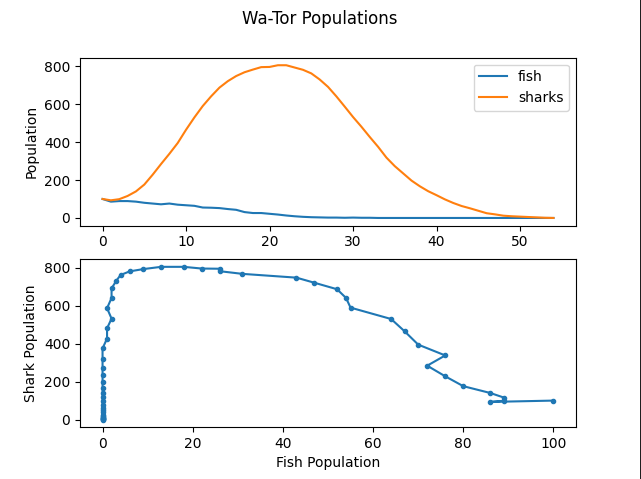
\includegraphics[width=0.6\textwidth]{figure1.png}
  \caption{\label{fig:figure1}
  Outcome one when \emph{energy\_gain} has the highest step with a random distribution.
  }
  \end{center}
\end{figure}

Likewise, with a discrete distribution where the population is grouped together, one can get the same results.

\begin{figure}[!htbp]
  \begin{center}
  \item[]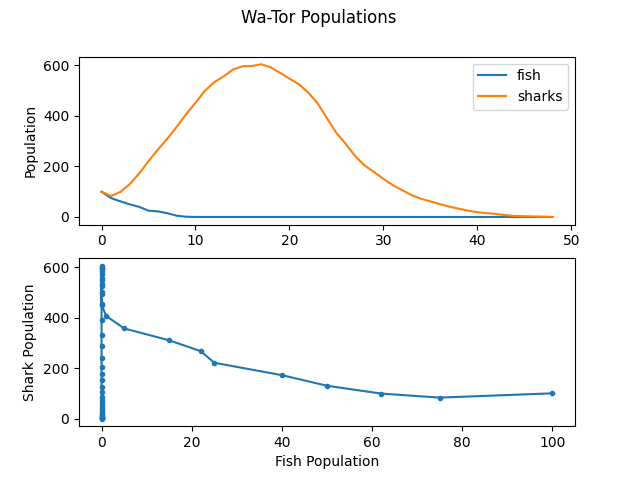
\includegraphics[width=0.6\textwidth]{figure2.png}
  \caption{\label{fig:figure2}
  Outcome one when \emph{energy\_gain} has the highest step with a discrete distribution.
  }
  \end{center}
\end{figure}

This situation is reasonable as the rate at which the sharks consume the fish is high, then the fish die out faster than they can reproduce and the sharks die due to the lack of fish to eat. 
The only difference is the rate at which this happens is different between the distributions, as shown in both Fig. \ref{fig:figure1} and Fig. \ref{fig:figure2} with their respective Shark vs. Fish population graphs.

When the amount of sharks initially (\emph{initial\_sharks}) is at a high step then the sharks will eat all the fish, but at a faster rate. 
However, this only occurs when the population is randomly distributed as there are enough fish to repopulate during the discrete simulation.

\begin{figure}[h!tbp]
  \begin{center}
  \item[]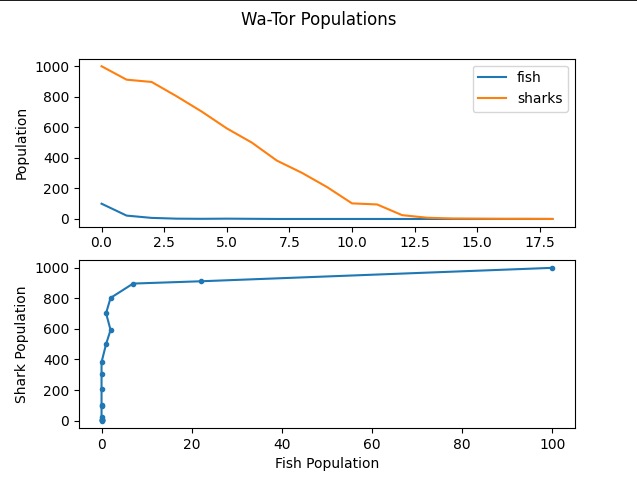
\includegraphics[width=0.6\textwidth]{figure3.png}
  \caption{\label{fig:figure3}
  Outcome one when \emph{initial\_sharks} has the highest step with a random distribution.
  }
  \end{center}
\end{figure}

The outcome where the fish population grows without restriction is the second outcome and is common when there are fish remaining in the simulation when there are no sharks. 
This is common when the \emph{energy\_gain} step is less than the \emph{breed\_time} of the fish population and the breed rate of the sharks' \emph{breed\_energy}.

\begin{figure}[h!tbp]
  \begin{center}
  \item[]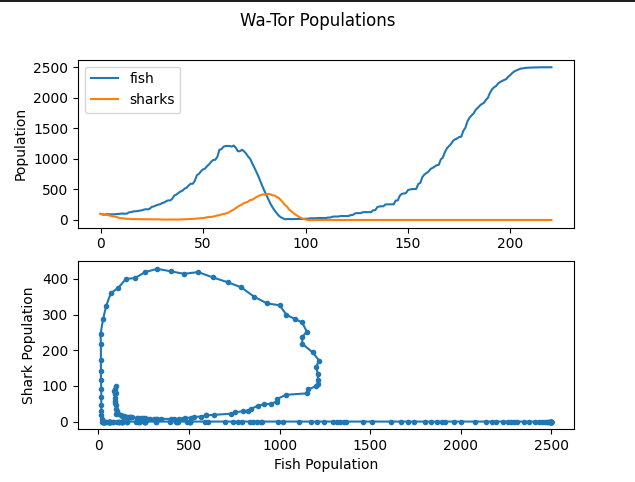
\includegraphics[width=0.6\textwidth]{figure4.png}
  \caption{\label{fig:figure4}
  Outcome two when \emph{energy\_gain} has the lowest step with a random distribution.
  }
  \end{center}
\end{figure}

\begin{figure}[h!tbp]
  \begin{center}
  \item[]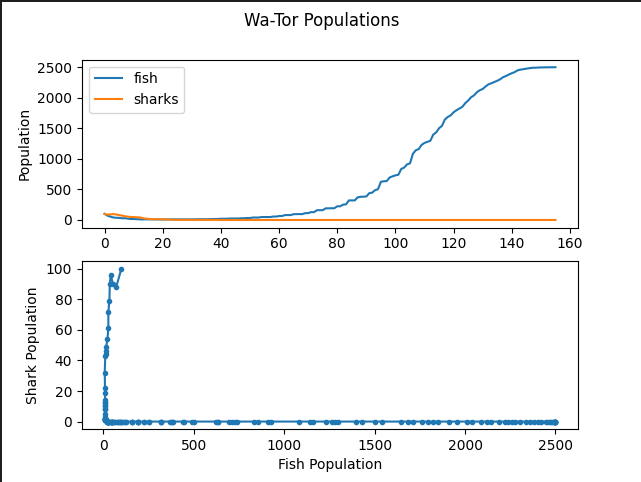
\includegraphics[width=0.6\textwidth]{figure5.png}
  \caption{\label{fig:figure5}
  Outcome two when \emph{energy\_gain} has the lowest step with a random distribution.
  }
  \end{center}
\end{figure}

In these cases, regardless of the type of distribution, the sharks will die out but the fish will continue to grow. 
The only difference between the distributions is the Shark vs. Fish population graphs in Fig. \ref{fig:figure4} and Fig. \ref{fig:figure5}; both have different rates at which the fish will eventually grow continuously with no interference. 
The same outcome occurs when the number of fish initially (\emph{inital\_fish}) is greater than that of the initial shark population. 
This situation is reasonable as the sharks will eventually run out of spaces to move as they eat the fish around them, creating a situation where they die out but the fish population still grows.

Similarly, if the fish population is below the amount of sharks initially, there will not be enough fish for the sharks to eat. 
However, the distribution of the fish population creates a situation where there will still be fish left. 
This happens in both scenarios with random and discrete distribution.

\begin{figure}[h!tbp]
  \begin{center}
  \item[]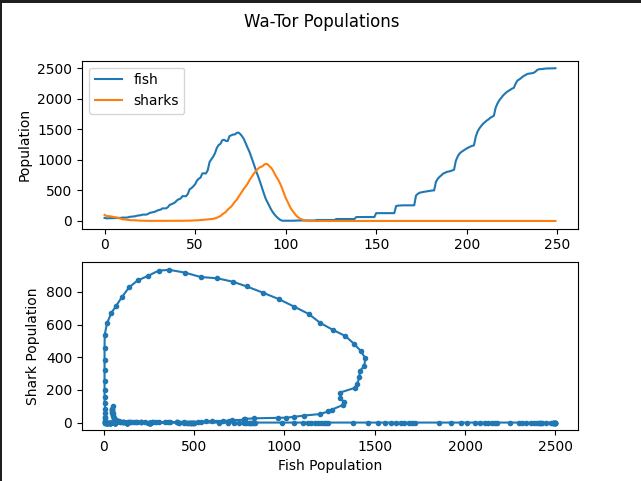
\includegraphics[width=0.6\textwidth]{figure6.png}
  \caption{\label{fig:figure6}
  Outcome two when \emph{energy\_gain} has the lowest step with a random distribution.
  }
  \end{center}
\end{figure}

\begin{figure}[h!tbp]
  \begin{center}
  \item[]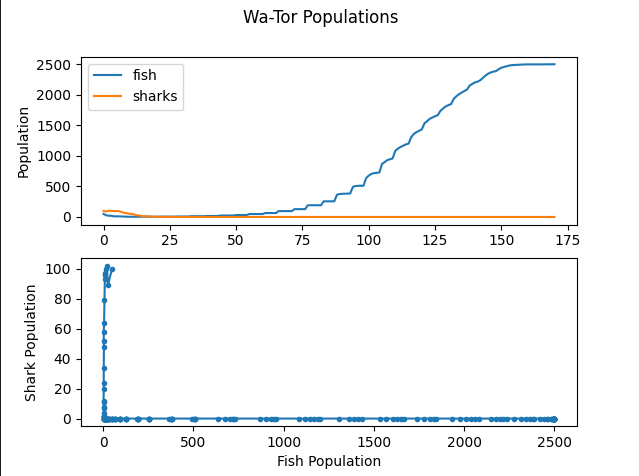
\includegraphics[width=0.6\textwidth]{figure7.png}
  \caption{\label{fig:figure7}
  Outcome two when \emph{energy\_gain} has the lowest step with a discrete distribution.
  }
  \end{center}
\end{figure}

Both Fig \ref{fig:figure6} and Fig \ref{fig:figure7} have the same outcome (the fish continue to grow), but the rates at which this happens varies based on the population distribution as shown on the Shark v. Fish Population graphs of both figures.


The situations where the population oscillates between the fish and the shark population (i.e. situations of an ideal Lotka-Volterra model) can happen at different rates and are uncommon compared to the other two outcomes. 
Furthermore, there are in fact two oscillation types that can occur: one where the fish population and shark population will fluctuate at an equal rate, and another where the fish population will nearly be extinct, but will slightly fluctuate allowing for the amount of shark population to fluctuate at a higher peak than the fish population.

For the first situation out of this outcome, this could happen when the \emph{breed\_energy} variable is set at the correct step. 
Shown in the following figure, the \emph{breed\_energy} is set to 100 while the other default variables are set to 10. 
The number of fish and shark initially are the same set at a step of 100 with a random distribution.

\begin{figure}[h!tbp]
  \begin{center}
  \item[]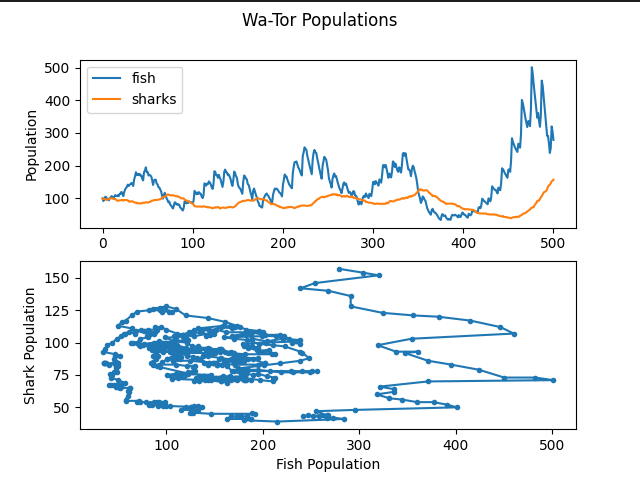
\includegraphics[width=0.6\textwidth]{figure8.png}
  \caption{\label{fig:figure8}
  Fluctuating population
  }
  \end{center}
\end{figure}

While this can happen with the parameters set, there is a chance at which this will not happen at all and the outcome where both populations die out will happen. 
If the time of the simulation increases, then this outcome will not happen and both populations will die out.

The second fluctuating outcome can happen when the starting energy (\emph{start\_energy}) is higher than the default variables.

\begin{figure}[h!tbp]
  \begin{center}
  \item[]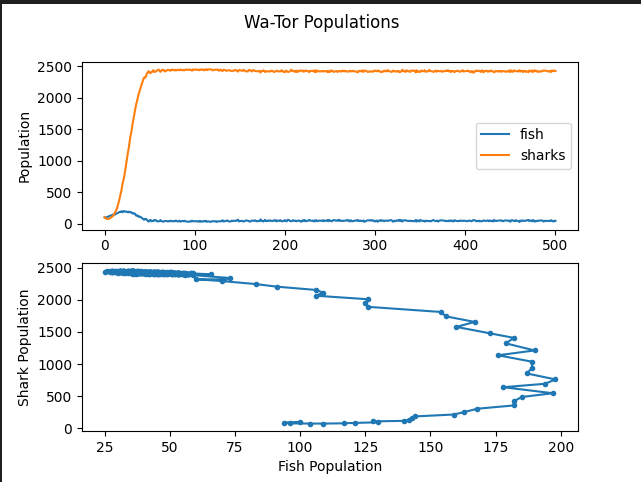
\includegraphics[width=0.6\textwidth]{figure9.png}
  \caption{\label{fig:figure9}
  Fluctuating population, random
  }
  \end{center}
\end{figure}

\begin{figure}[h!tbp]
  \begin{center}
  \item[]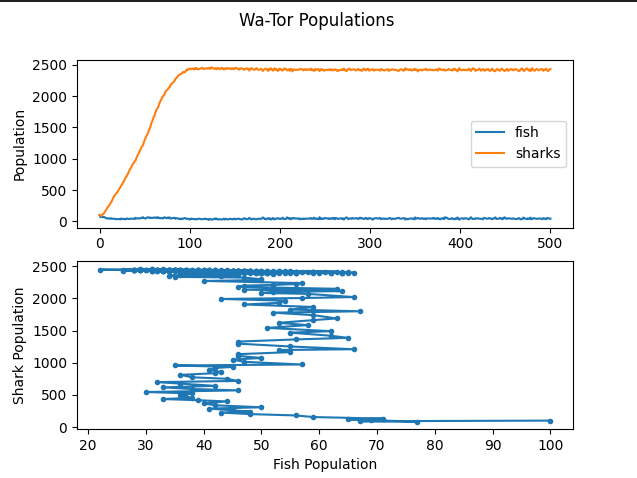
\includegraphics[width=0.6\textwidth]{figure10.png}
  \caption{\label{fig:figure10}
  Fluctuating population, discrete
  }
  \end{center}
\end{figure}

In this sub-outcome, the population of the fish becomes nearly extinct, but there is a small enough fish population that allows the shark population to grow to a certain point whilst still being continuous.

It seems that the base simulation works best when the shark population does not grow too quickly but fast enough that the sharks are able to moderate the fish population given a set range for the main parameters. 
The simulation becomes more consistent when the rate at which fish reproduce is high enough to sustain the shark population. 
Along with this, we must maintain the proper ratio of fish to sharks with respect to the size of the “play area”. 
For most scenarios tested, we found that the shark population was usually the culprit more often than not when observing an early termination. 
We fix this by reducing the rate at which sharks reproduce, by either reducing the energy gained from eating a fish – which is our $b$ constant from the provided equation – or by adjusting the energy requirement to reproduce so that a new shark must eat more than 2 fish to reproduce. 
Keeping a low breed time for the fish allowed for the population to bounce back if the shark population over-monitored and easily settle into the steady state solution.

\begin{figure}[h!tbp]
  \begin{center}
  \item[]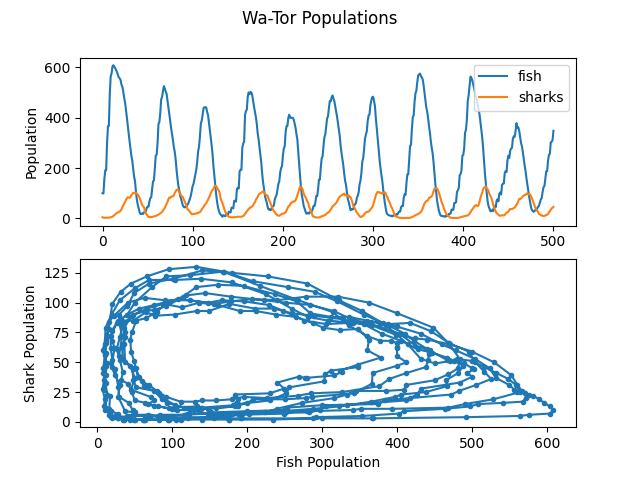
\includegraphics[width=0.48\textwidth]{figure11.png}
  \caption{\label{fig:figure11}
  Play area 25x25, breedtime = 2, energy gain = 2, breed energy = 9, sharks = 5, fish = 100, 500 steps
  }
  \end{center}
\end{figure}

\begin{figure}[h!tbp]
  \begin{center}
  \item[]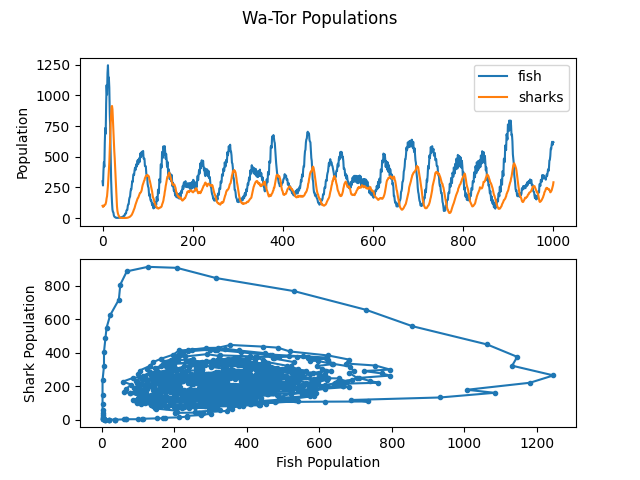
\includegraphics[width=0.48\textwidth]{figure12.png}
  \caption{\label{fig:figure12}
  Play area 25x25, breedtime = 2, energy gain = 4, breed energy = 12, sharks = 100, fish = 300, 1000 steps
  }
  \end{center}
\end{figure}

\begin{figure}[h!tbp]
  \begin{center}
  \item[]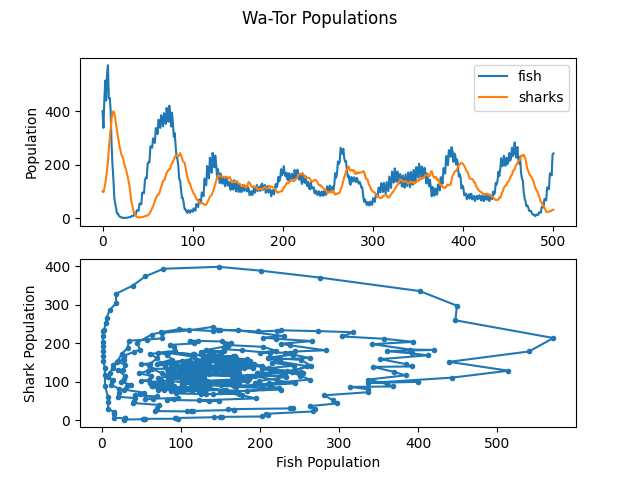
\includegraphics[width=0.48\textwidth]{figure13.png}
  \caption{\label{fig:figure13}
  Play area 40x40, breedtime = 2, energy gain = 5, breed energy = 15, sharks = 100, fish = 400, 500 steps
  }
  \end{center}
\end{figure}

\pagebreak

\subtitle{\textbf{Relationship Between Main Simulation Parameters and Lotka-Volterra Constants}}

The \emph{energy\_gain} variable is related to the Lotka-Volterra model parameters $a$ and $b$ (the decay rate and the growth rate of the sharks). 
Theoretically, if the growth of the predator population reaches a point where it is high enough that the prey population dies out, then the predator population will also die out due to starvation. 
This is reasonable since the decay rate of the predator population is proportional to the population of the shark population, and the growth rate of the population is proportional to both the amount of predators and prey.

Now considering the simulation, there are two possible outcomes when changing the \emph{energy\_gain} in the program.

\begin{figure}[h!tbp]
  \begin{center}
  \item[]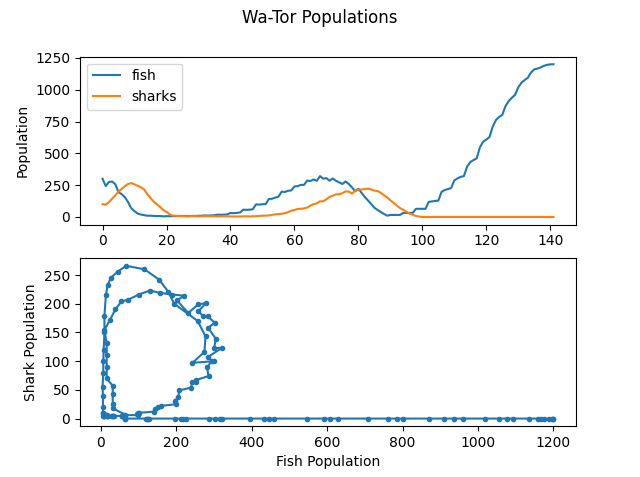
\includegraphics[width=0.5\textwidth]{figure14.png}
  \caption{\label{fig:figure14}
  energy\_gain, step of 5
  }
  \end{center}
\end{figure}

\begin{figure}[h!tbp]
  \begin{center}
  \item[]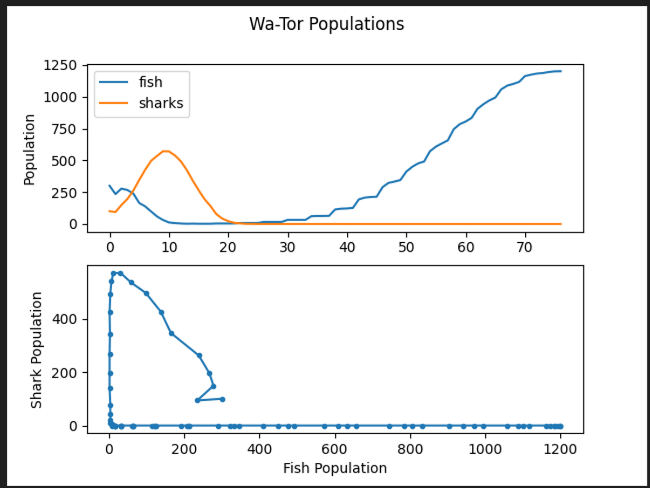
\includegraphics[width=0.5\textwidth]{figure15.png}
  \caption{\label{fig:figure15}
  energy\_gain, step of 10
  }
  \end{center}
\end{figure}

\begin{figure}[h!tbp]
  \begin{center}
  \item[]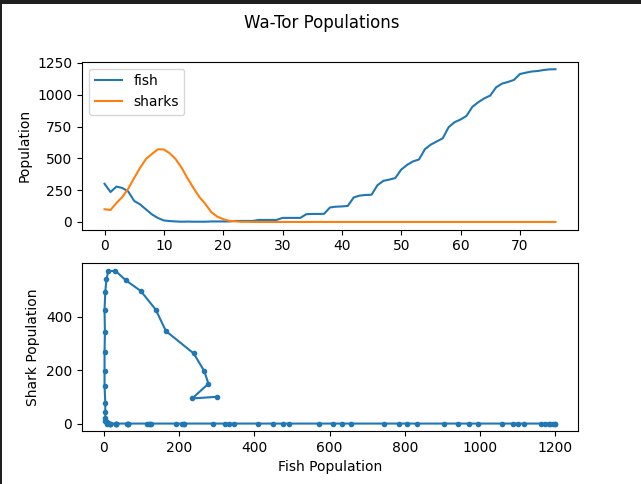
\includegraphics[width=0.5\textwidth]{figure16.png}
  \caption{\label{fig:figure16}
  energy\_gain, step of 15
  }
  \end{center}
\end{figure}

As observed, when the energy gained by the shark increases and is greater than that of the growth rate of the fish, the shark will eventually eat all the fish at a faster rate than the growth of the fish population. 
Eventually, the fish population will decay to zero and the shark population reaches its maximum population. 
It is at this point that the shark population decays toward zero as there are no more prey -- this leads to the growth of fish in the system without the sharks.

Now when the growth rate of the fish (\emph{breed\_time}) is greater than that of the \emph{energy\_gain} step. 
The \emph{breed\_time} will be set to 20 and the \emph{energy\_gain} will be decremented by a step of 5 starting at a step of 20.

\begin{figure}[h!tbp]
  \begin{center}
  \item[]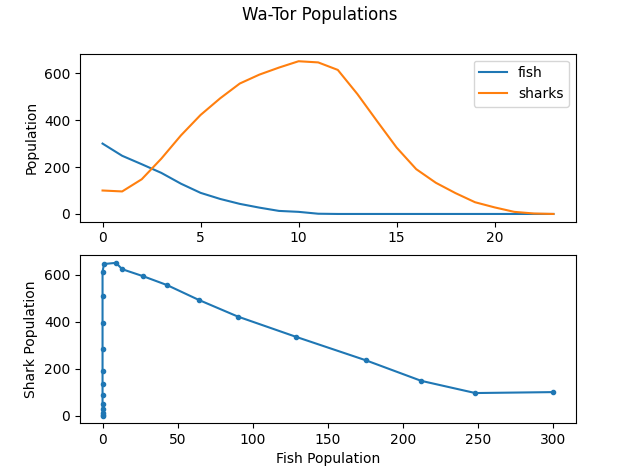
\includegraphics[width=0.5\textwidth]{figure17.png}
  \caption{\label{fig:figure17}
  energy\_gain, step of 20
  }
  \end{center}
\end{figure}

\begin{figure}[h!tbp]
  \begin{center}
  \item[]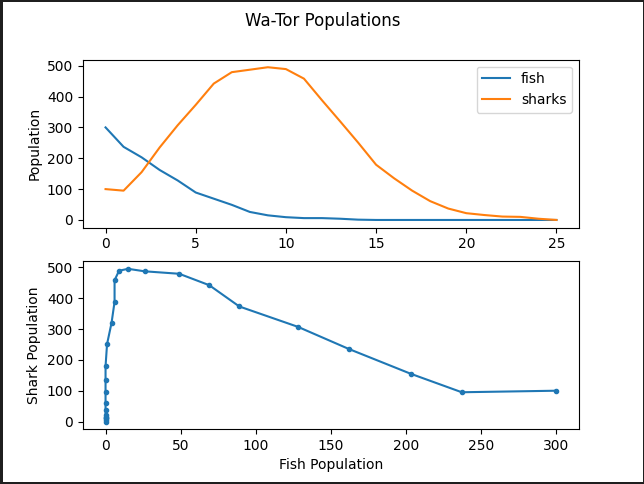
\includegraphics[width=0.5\textwidth]{figure18.png}
  \caption{\label{fig:figure18}
  energy\_gain, step of 15
  }
  \end{center}
\end{figure}

\begin{figure}[h!tbp]
  \begin{center}
  \item[]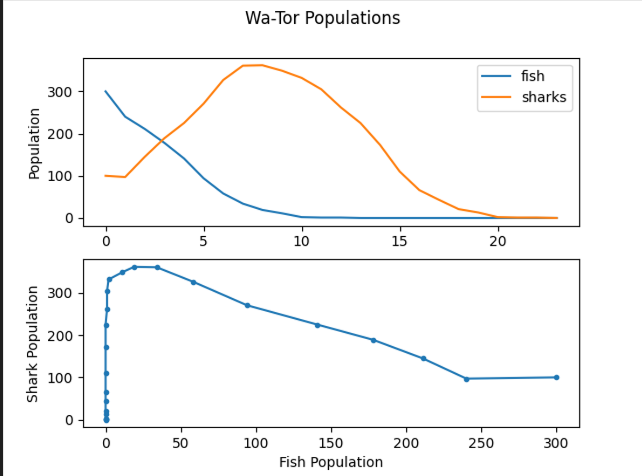
\includegraphics[width=0.5\textwidth]{figure19.png}
  \caption{\label{fig:figure19}
  energy\_gain, step of 10
  }
  \end{center}
\end{figure}

\begin{figure}[h!tbp]
  \begin{center}
  \item[]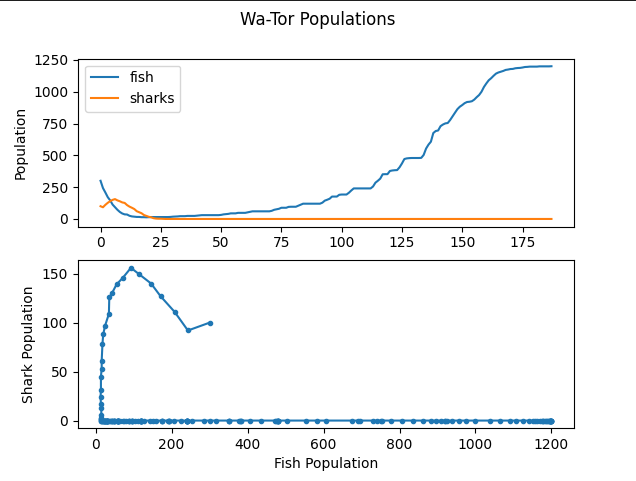
\includegraphics[width=0.5\textwidth]{figure20.png}
  \caption{\label{fig:figure20}
  energy\_gain, step of 5
  }
  \end{center}
\end{figure}

Similar to the first case, the shark population will eventually reach a maximum population size, but decay due to there being no prey in the system. 
However, in the first three figures, both the shark population and fish population reach zero at a certain point. 
This is plausible as the rate at which the shark population reaches its maximum decreases with the step size of the \emph{energy\_gain} variable. 
This creates a point at which the shark population reaches its peak, but there will still be a small amount of the fish population that exists. 
Therefore, as the shark population reaches zero, there would still be some fish in the system to be able to grow without interference from the sharks.

However, these outcomes can also depend on the distribution of the system (i.e. if the distribution is random). 
These examples used a random distribution, but the relationship was still consistent between either of these two outcomes. 
When using a more discrete distribution between the sharks and fish (they are grouped together), the outcome where the fish starts to grow after all sharks die out happens.

Breed time affects the fish population growth rate. 
The rate is inversely proportional to the entered value. 
Therefore, a smaller number will equate to a faster population growth, and vice versa. 
This constant also affects predator growth rate, because the fish will fill up all of the play area, and the sharks will easily achieve the reproduction requirement to continue growing. 
Theoretically we expect, at the low extreme, the fish population to grow very quickly with the shark population following by 90 degrees, but the fish population caps, and the sharks over hunt the fish population. 
The shark population dies out due to resource depletion, and the fish rebound with little to no predators around to moderate the population. 
In the high extreme, we expect the shark population to over hunt the fish population, and the fish population does not rebound, due to low reproduction rates.

\begin{figure}[h!tbp]
  \begin{center}
  \item[]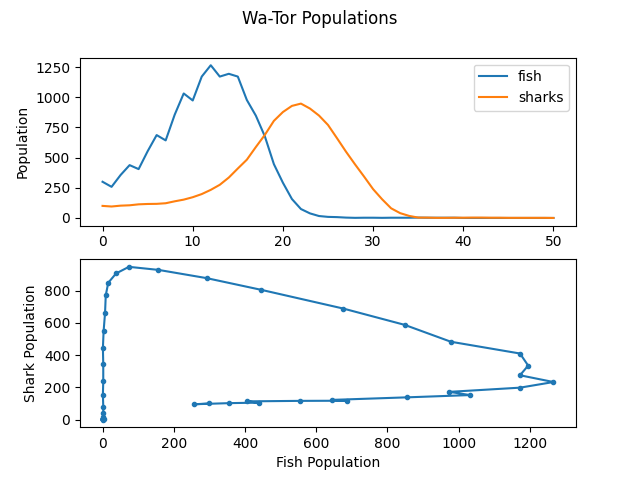
\includegraphics[width=0.5\textwidth]{figure21.png}
  \caption{\label{fig:figure21}
  breed time = 2
  }
  \end{center}
\end{figure}

\begin{figure}[h!tbp]
  \begin{center}
  \item[]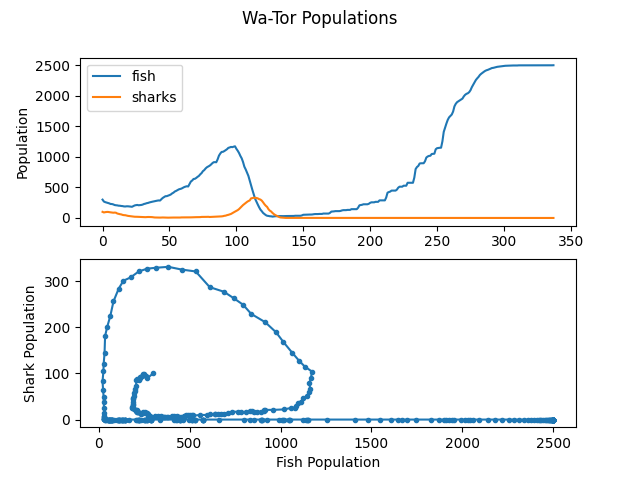
\includegraphics[width=0.5\textwidth]{figure22.png}
  \caption{\label{fig:figure22}
  breed time = 20
  }
  \end{center}
\end{figure}

We believe that the breed energy variable is in control of the $d$ constant, since this constant only affects how many sharks are around at a given time. 
The prime example of having a low breed energy is when the shark population dies out due to having insufficient food resources to be able to breed, because of a rapidly expanding shark population as seen in the figure below.

An excellent example of having a high breed energy is when the sharks and fish coexist, but the fish population greatly outnumbers due to the sharks not being able to reproduce quick enough to manage the fish population. 
The other common outcome is when the shark population dies out due to not being able to breed fast enough to sustain a population. 
Theoretically, we anticipate that when the lower the breed energy, the more often the sharks will reproduce, and the higher the value, the sharks will reproduce less often.

\begin{figure}[h!tbp]
  \begin{center}
  \item[]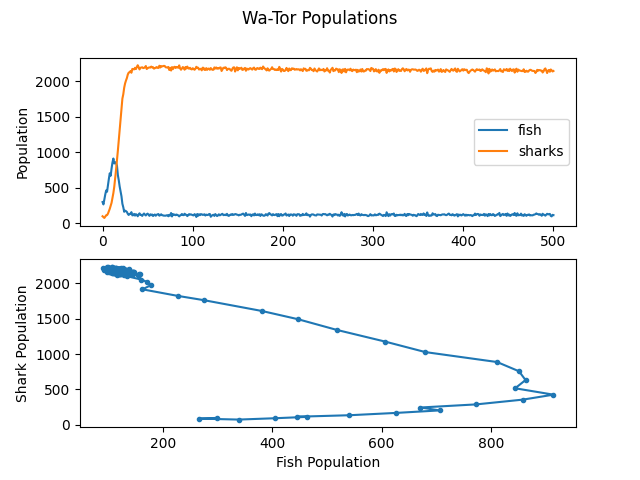
\includegraphics[width=0.5\textwidth]{figure23.png}
  \caption{\label{fig:figure23}
  Play area 50x50, breedtime = 3, energy gain = 4, breed energy = 4, sharks = 100, fish = 300, 500 steps
  }
  \end{center}
\end{figure}

\begin{figure}[h!tbp]
  \begin{center}
  \item[]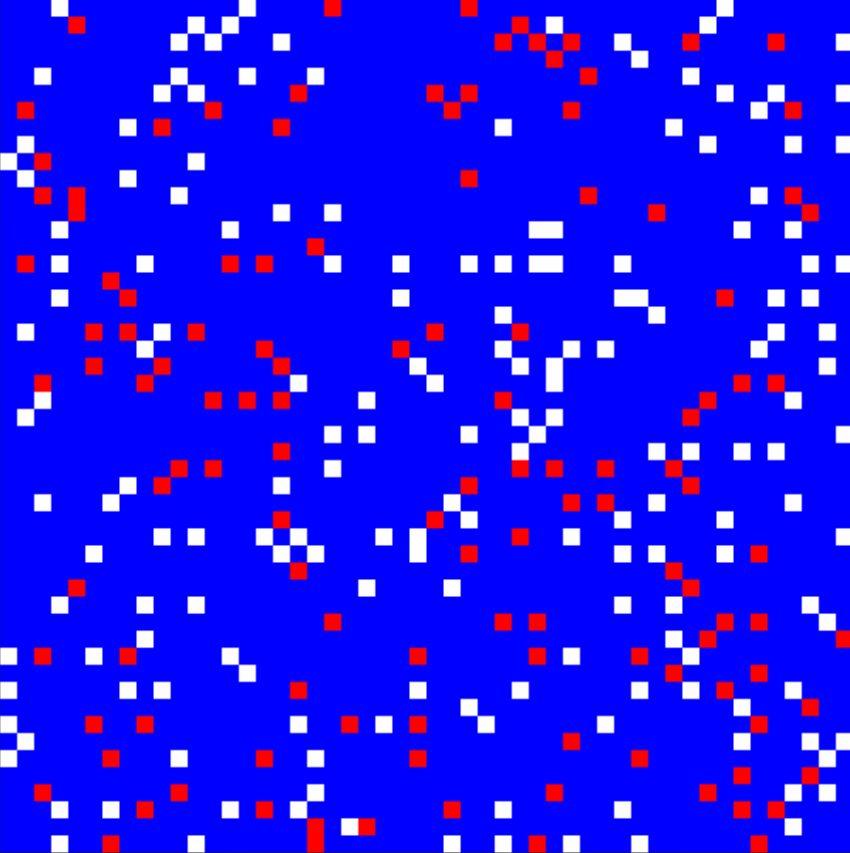
\includegraphics[width=0.5\textwidth]{figure24.png}
  \caption{\label{fig:figure24}
  GIF still of play area 50x50, breedtime = 3, energy gain = 4, breed energy = 4, sharks = 100, fish = 300, 500 steps
  }
  \end{center}
\end{figure}

\pagebreak

\subtitle{\textbf{Effects of Other Parameters}}

Start energy determines the starting energy level of the sharks when spawned in, and by extension affects the initial breed time, because the amount of energy necessary to reproduce is smaller for the first reproduction cycle. 
This can be observed when comparing extreme cases of 0 starting energy, and requiring one energy to reproduce. 
Therefore, the starting energy is a transient parameter.

\begin{figure}[h!tbp]
  \begin{center}
  \item[]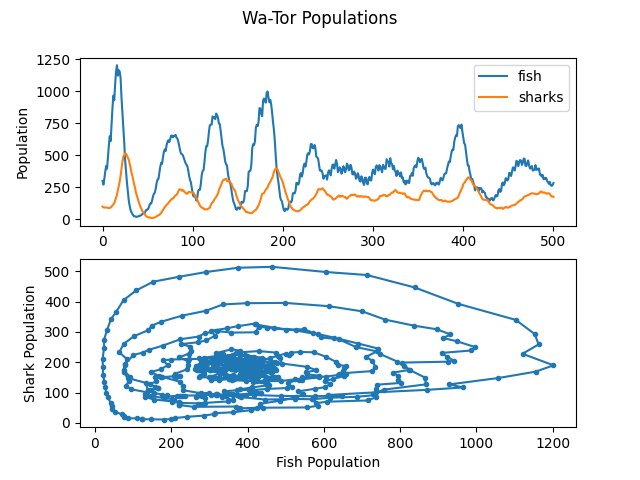
\includegraphics[width=0.5\textwidth]{figure25.png}
  \caption{\label{fig:figure25}
  Here, the amplitude is not as high and initial amplitude is much smaller than the next figure
  }
  \end{center}
\end{figure}

\begin{figure}[h!tbp]
  \begin{center}
  \item[]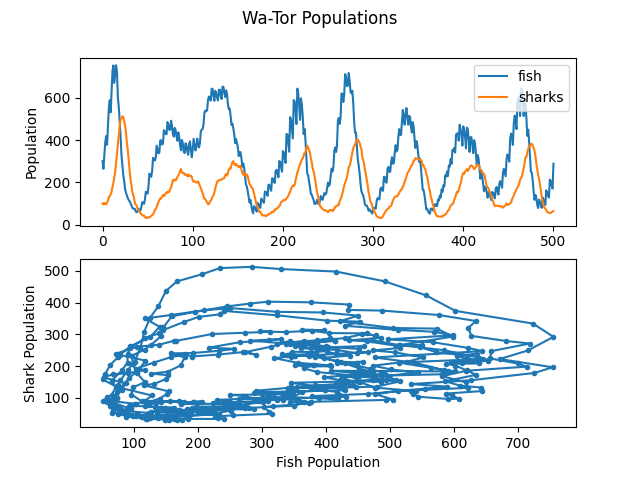
\includegraphics[width=0.5\textwidth]{figure26.png}
  \caption{\label{fig:figure26}
  Shark population amplitude is higher as a result of greater start energy
  }
  \end{center}
\end{figure}

Steps determines how long the simulation will continue on for, and is good to see which parameters are short-term effects or long-term effects (transient or a steady-state parameter).

Initial sharks and fish determine how many of each animal we want at the beginning of the simulation. 
If we have a larger ratio of sharks to fish, then the simulation is more likely to reach an early termination due to the fish population being hunted down to zero. 
If this does not occur then we have a good ratio, otherwise we have a small ratio of sharks to fish, and both populations continue onward.

We have experienced success with varying population sizes, but believe that the simulation works best when the ratio of fish to sharks had a range of 5\% - 40\%.

\begin{figure}[h!tbp]
  \begin{center}
  \item[]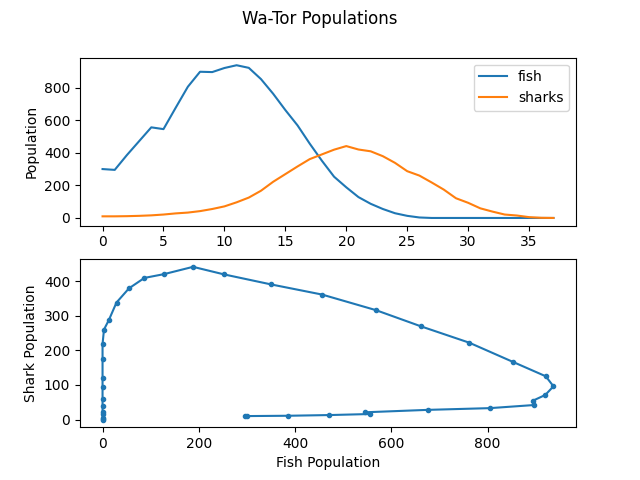
\includegraphics[width=0.5\textwidth]{figure27.png}
  \caption{\label{fig:figure27}
  Early termination due to fish population being hunted down to zero
  }
  \end{center}
\end{figure}

The basic setup setting determines if the distribution is random or not. 
The non-basic setup means that the sharks and fish are organized in a circle, with the sharks in the middle and fish surrounding the sharks as seen in Fig \ref{fig:figure28}.

\begin{figure}[h!tbp]
  \begin{center}
  \item[]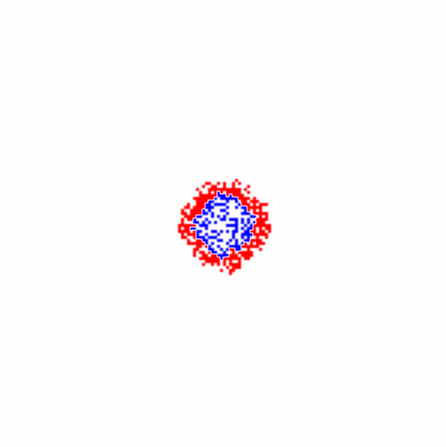
\includegraphics[width=0.5\textwidth]{figure28.png}
  \caption{\label{fig:figure28}
  GIF still of the non-basic setup
  }
  \end{center}
\end{figure}

\begin{figure}[h!tbp]
  \begin{center}
  \item[]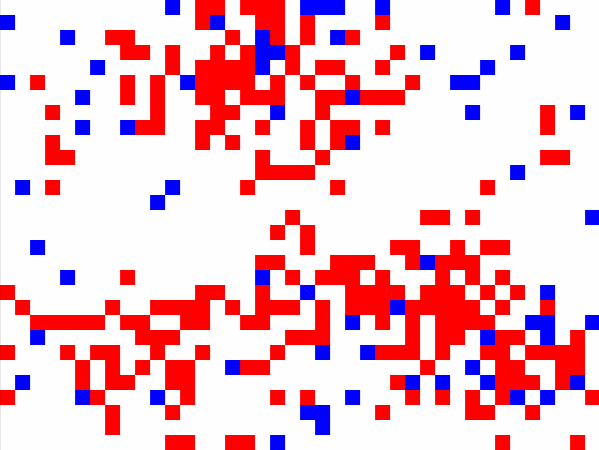
\includegraphics[width=0.5\textwidth]{figure29.png}
  \caption{\label{fig:figure29}
  GIF still of the basic (random) setup
  }
  \end{center}
\end{figure}

This leads the sharks to expand outward and hopefully some of the fish make it into the center, then both populations oscillate back and forth. 
This works just about every time, but is unrealistic. 
The random set-up is more realistic because of how insufficient the basic setup is for emulating groupings of fish and sharks.

\begin{figure}[h!tbp]
  \begin{center}
  \item[]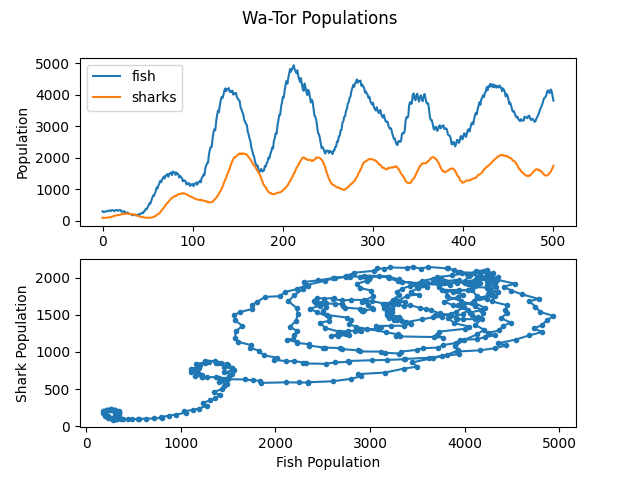
\includegraphics[width=0.5\textwidth]{figure30.png}
  \caption{\label{fig:figure30}
  Non-basic setup
  }
  \end{center}
\end{figure}

\pagebreak

%%%%%%%%%%%%%%%%%%%% Extension %%%%%%%%%%%%%%%%%%%%
\section{Extension}


The modification we decided to implement was more realistic fish behavior. 
This was done by adding some lines of code in the part of the simulation that implements the fish’s movement that prevent the fish from moving into spots that are adjacent to those occupied by sharks. 
In order to allow the fish to scan adjacent locations for sharks, we first needed to create a function that checks for spaces that are occupied by sharks, similar to the removeoccupied function (the one that checks for empty spaces) and the findfishoccupied function (the one that checks for spaces occupied by fish). 
Thus, we named our new function findsharkoccupied, and the implementation was almost the exact same as the aforementioned two functions. 
In the simulation, empty spaces held the value zero, spaces occupied by fish held a positive value, and spaces occupied by sharks held a negative value. 
The first two functions checked each location for the value of zero or a positive value, respectively, before adding it to the list of available/occupied spaces – consequently, this new function checked each location for a negative value before adding it to the list of occupied spaces.


\begin{figure}[htbp]
  \begin{center}
  \item[]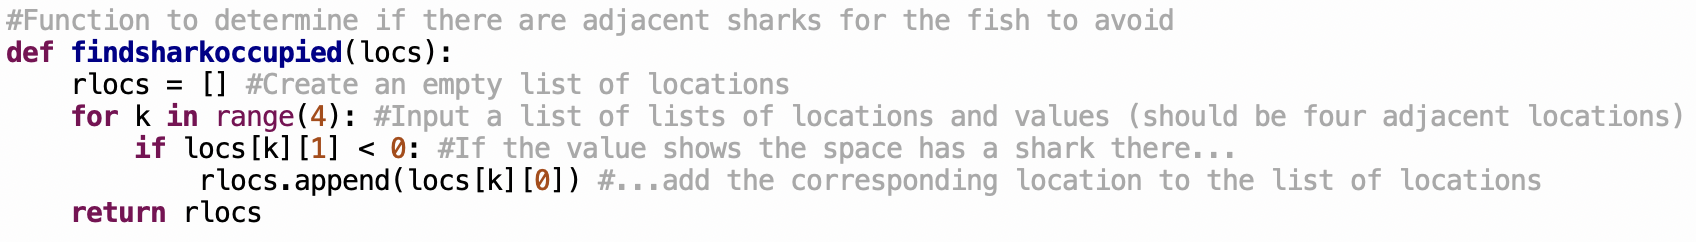
\includegraphics[width=0.95\textwidth]{findSharkOccupied.png}
  \caption{\label{fig:findSharkOccupied}
  Screenshot of the code for the function to find adjacent spaces occupied by sharks
  }
  \end{center}
\end{figure}


The next step was to actually use this function in the main function of the simulation to prevent the fish from being suicidal. 
The original code created two lists, oldlocs and newlocs, which check for adjacent empty spaces for the fish to move into using the removeoccupied function. 
It then found the intersection of these lists, placing it into a new list called availlocs. 
This new list held all of the empty adjacent spaces that the fish could move into, and if there were any available options, then the fish would choose one at random and move into it. 
In order to make our fish more realistic, however, we would need them to move into adjacent spaces that are empty but also not adjacent to a shark. 
Thus, we created four new lists: oldsharklocs, which scanned through the old array’s adjacent locations for sharks; newsharklocs, which scanned through the new array’s adjacent locations for sharks; sharklocs, which was the intersection of the former two lists; and actualavaillocs, the list of elements that were contained in availlocs but not in sharklocs. 
Instead of checking availlocs for available options to move into, the fish now checked actualavaillocs to satisfy the modification’s condition. 
Below is a screenshot of the modified code:


\begin{figure}[htbp]
  \begin{center}
  \item[]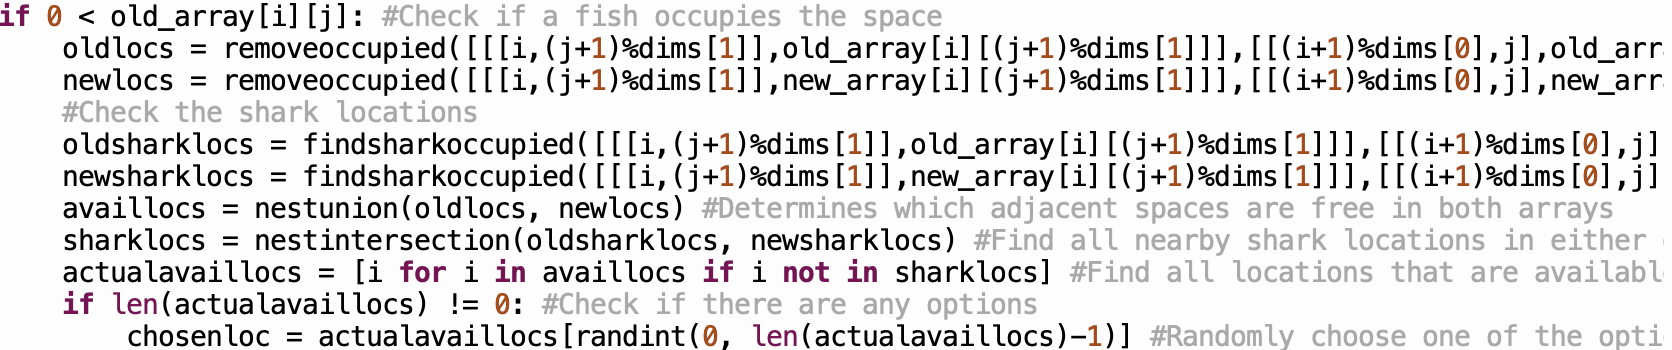
\includegraphics[width=0.95\textwidth]{modifiedFishMovement.png}
  \caption{\label{fig:modifiedFishMovement}
  Screenshot of the code used to modify the fish’s movement
  }
  \end{center}
\end{figure}


After running the simulation a few times with the rest of the parameters set to their defaults, some distinct trends were observed that differentiated this version from the original. 
In every run, the population of fish is much higher than that of the sharks, and the rises and drops in the graphs are not as dramatic as the original runs. 
These changes in population are also less periodic and seem more sporadic. 
This could be explained by the fact that the fish were less likely to be eaten at each step now, so they could maintain a more steady population with less sudden changes. 
In each of the runs, there was also an initial drop in population for both the fish and sharks, but then the fish would rise in population while the sharks would remain at a much lower population. 
This may be a result of the random initial distribution of the fish and shark populations – after “settling down”, the fish are able to repopulate and evade the sharks better while the sharks have a harder time catching up to them.

This modified simulation still bears some similarities to the original one, though. 
The populations do not remain constant, and there is some up and down movement, albeit not as pronounced as the original. 
The graphs also show how the shark population still lags 90 degrees behind the fish population, which is expected considering the sharks still have to wait for the fish to move and reproduce first before they can move. 
Below are some plots which exhibit the aforementioned behaviors:


\begin{figure}[htbp]
  \begin{center}
  \item[]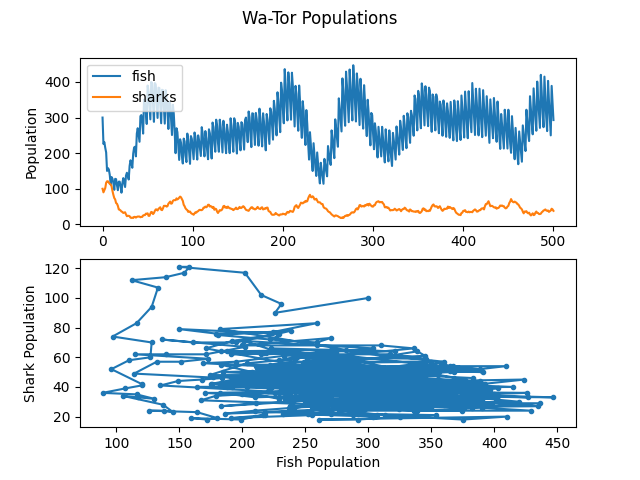
\includegraphics[width=0.6\textwidth]{run4plots.png}
  \end{center}
  \caption{\label{fig:run4plots}
  Modified Simulation Run 1
  }
\end{figure}

\begin{figure}[htbp]
  \begin{center}
  \item[]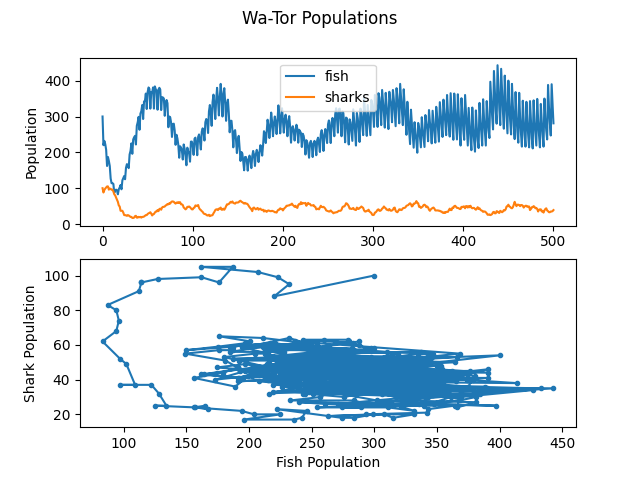
\includegraphics[width=0.6\textwidth]{run5plots.png}
  \end{center}
  \caption{\label{fig:run5plots}
  Modified Simulation Run 2
  }
\end{figure}

\begin{figure}[htbp]
  \begin{center}
  \item[]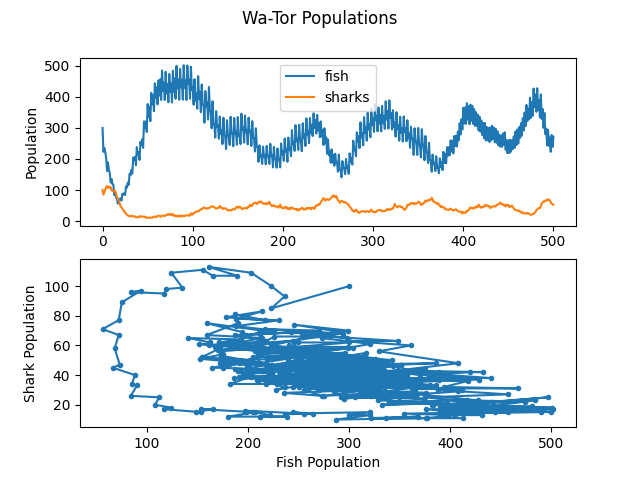
\includegraphics[width=0.6\textwidth]{run6plots.png}
  \end{center}
  \caption{\label{fig:run6plots}
  Modified Simulation Run 3
  }
\end{figure}

\end{document}
%%%%%%%%%%%%%%%%%%%% Document Ends %%%%%%%%%%%%%%%%%%%%
